\documentclass[11pt]{article}
\usepackage{fullpage,graphicx}
\usepackage{rotating}
\parskip=10pt \parindent=0pt

\begin{document}
\section*{Including Landscape Figures and Tables in a \LaTeX\ Document}
To insert landscape figures or tables, you'll need two packages, 
\texttt{graphicx} and \texttt{rotating}, which are included with most 
\TeX/\LaTeX\ distributions.  
The \texttt{graphicx} package defines a new command called 
\verb+\includegraphics+ that enables you to include (and scale, 
if necessary) an imported graphic. 
Note that \LaTeX\ plus \texttt{dvips} requires imported graphics to be in 
encapulated PostScript (EPS) format, while pdf\LaTeX\ accepts PDF, JPEG, 
or PNG formats but \textit{not} EPS. (The conversion programs 
\texttt{epstopdf} and \texttt{jpeg2ps} are very useful.)
The \texttt{rotating} package provides two new environments,
\texttt{sidewaysfigure} and \texttt{sidewaystable}, which you use in
place of the standard \LaTeX\ environments \texttt{figure} and 
\texttt{table}. The sideways environments always put the landscape 
table or figure on a page by itself. 

\textbf{\large Documentation}\\[2pt]
Full documentation for the \texttt{rotating} package is in the book 
the \textit{The \LaTeX\ Companion} by Mittlebach \& Goossens. 
Documentation for the \texttt{graphicx} package is in the file
\texttt{grfguide.pdf}. Under TeXLive 2005 this file is 
in the folder: 
    \verb+C:\TeXLive2005\texmf-dist\doc\latex\graphics\+.
On other systems, it will be in a similar location. 
The material on including graphics is in Section 4.4.
 
Another useful document is \textit{Using Imported Graphics in \LaTeX2e}, 
a large PDF document by Keith Reckdahl of Stanford University. 
It includes all you would ever want to know with many examples. 
You can find it at 
\verb+http://www.ctan.org/tex-archive/info/epslatex.pdf+.

\textbf{\large Viewing the Result}\\[2pt] 
If you use pdf\LaTeX, the resulting PDF file should 
display everything properly.
If you are running \LaTeX\ to process your file, most of the time the 
previewer will be able to display the included PostScript
graphics (by calling the \verb+ghostscript+ program).  
However, landscape tables will not display correctly, and if the
graphic is in landscape orientation, it may not display properly.
To see a correct display, use \verb+dvips+ to put the output in a 
PostScript file and then use GSView to view it.  

To view the output from this document, which contains landscape figures 
and tables, look at either of the files \texttt{exrotating.ps} or 
\texttt{exrotating.pdf}. If you compare the output with the \LaTeX\ input 
(\texttt{exrotating.tex}), you'll see how the latex code generated
the resulting output. To try it yourself, copy \texttt{exrotating.tex} 
to your own directory, along with the graphics files \texttt{cat.eps}, 
\texttt{smokeblk.eps} and \texttt{cat.pdf}, \texttt{smokeblk.pdf}. 
Then either run \LaTeX\ followed by \texttt{dvips} or run pdf\LaTeX. 

\textbf{\large Examples} \\[2pt]
This file illustrates the use of both the \texttt{graphicx} and
\texttt{rotating} packages and can be processed either with pdf\LaTeX\ or
with \LaTeX\ plus \texttt{dvips}.  Note that, in the examples that follow,
the filename extension is purposely omitted in the 
\verb+\includegraphics+ commands. \LaTeX\ will look for files with the 
extension \texttt{.eps} and pdf\LaTeX\ will look for files with extensions 
\texttt{.pdf}, \texttt{.jpg} or \texttt{.png}. 
 
%%%%%%%%%%%%%%%%%%%%%%%%%%%%%  EXAMPLES  %%%%%%%%%%%%%%%%%%%%%%%%%%%%
% Portrait figure. \includegraphics will include either cat.eps or cat.pdf
\begin{figure}[b]   % the [b] specifies bottom of the page
\centering          % this centers everything inside the figure environment

\includegraphics{cat}
\caption{Here is a very small picture of a cat.}
\end{figure}

% a landscape figure which scales and rotates the file cat.eps or cat.pdf
\begin{sidewaysfigure}
\centering

\includegraphics[height=6in]{cat}
\caption{This is a stretched out cat to fill up the landscape page.}
\end{sidewaysfigure}
 
% A landscape table
\begin{sidewaystable}
\caption{A Very Wide Table}  
\bigskip
\centering  
  \begin{tabular}{|l|l|l|l|l|l|p{2.5in}|}  
  \hline  
  \multicolumn{6}{|c|}{Text in columns 1 through 6}   
        & A paragraph 2.5 inches wide \\  
  \hline  
  Column 1 & Column 2 & Column 3 & Column 4 & Column 5 & Column 6
                      & This text is a paragraph.  It will wrap  
                      around to the next line if necessary. \\  
  Column 1 & Column 2 & Column 3 & Column 4 & Column 5 & Column 6
                      & The paragraph column \\  
  \hline  
  \end{tabular}  
\end{sidewaystable}

% figure for landscape page
% The graphic is in the file smokeblk.eps or smokeblk.pdf
%
\begin{sidewaysfigure}
\centering
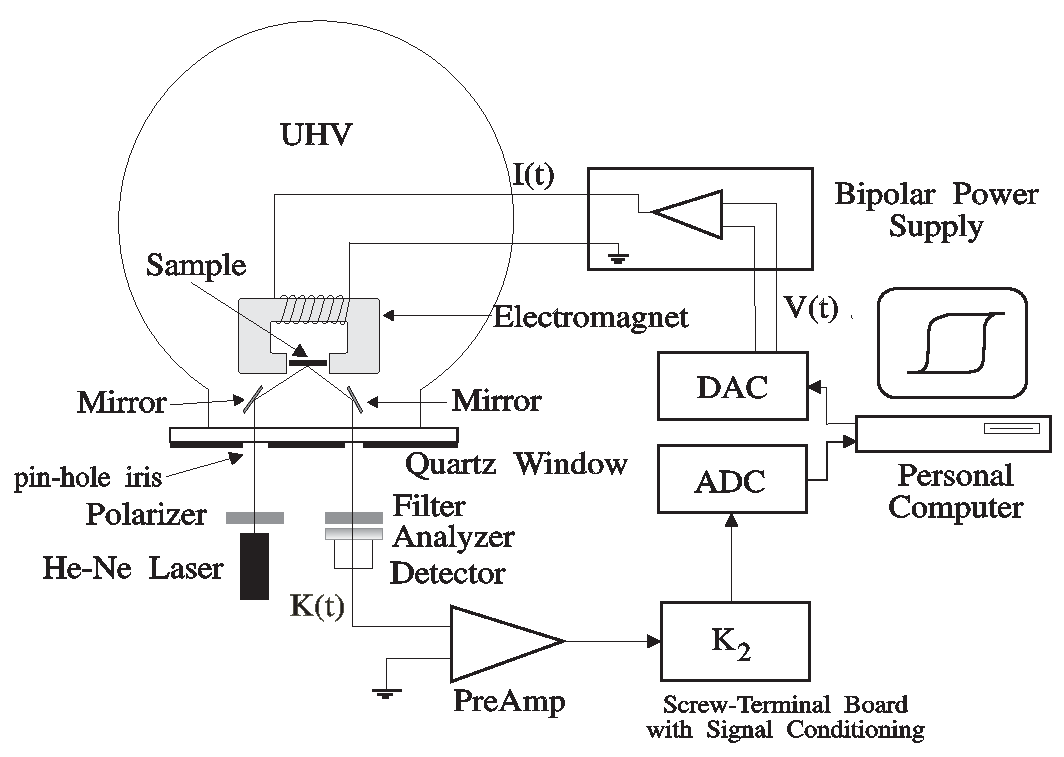
\includegraphics{smokeblk}
\caption{The Block diagram of the SMOKE setup showing the electromagnet,
bipolar power supply, optical components, preamplifier, photodetector, 
and a personal computer installed with an ADC and DAC board.}
\end{sidewaysfigure}
  
\end{document}
